\section{Softwarekonzept} \label{sec:softwarekonzept}

%TODO Besser beschreiben 
Die Beschreibung des Softwarekonzepts wird in 2 Sektionen unterteilt. Zuerst werden die in der Zieltabelle aufgeführten technischen und die graphischen Anforderungen beschrieben.  Anschliessend werden die Anforderungen an die Bedienung definiert. und zum Schluss werden die einzelnen Elemente der GUI, und somit die Bedienung erklärt.

\subsection{Programmablauf} \label{subsec:programmablauf}

Der folgende Programmablauf ist auf die Maximallösung bezogen. In dieser Lösung sind alle Wunschziele(Tabelle:\ref{tab:ziele}) vorhanden.

Nach dem Aufstarten des Programmes kann der Benutzer über die Programmoberfläche (\ref{fig:GUI} \nameref{fig:GUI}) seine Simulationen starten.
Am Anfang ist ein default Filter initialisiert. Dieser ist in der Filtertabelle eingetragen, jedoch sind die parasitären Filterparameter im Eingabefenster noch undefiniert. Der Benutzer kann diese nun definieren und die berechneten Einfügungsverluste von CM und DM des EMI-Filters werden im Plot dargestellt. Mit dem Button Add wird der Filter abgespeichert und ein neuer Filter kann definiert werden. Es können somit mehrere Filter gleichzeitig dargestellt werden. 

Um die Filter richtig zu verwalten ist es möglich in der Filtertabelle über die Checkbox einzelne Filter im Plot ein und auszublenden. Ebenfalls können sie spezifisch benannt werden. Der Plot und die einzelnen Kurven können mit einem Rechtsklick auf den CM/DM Plot individuell angepasst und auch exportiert werde. Wird ein Filter nicht mehr benötigt kann er in der Filtertabelle angewählt und mit dem Button Remove entfernt werden. Damit der Benutzer nicht jedesmal die Filterprofile einstellen muss, können diese über File/Save filterprofil in einer .txt Datei abgespeichert werden. Bei einem Neustart des Programmes kann über File/Load filterprofile die Filterprofile wieder geladen werden. 

Um die Auswirkungen einzelner parasitären Filterparameter besser zu analysieren, kann unter Simulation/Monte Carlo eine Monte Carlo Simulation gestartet werden. Es wird ein neues Fenster geöffnet in dem der Filterparameter, die Toleranz und die Anzahl Berechnungen eingestellt werden können. Jede Berechnung wird als einzelner Filter in die Filtertabelle geladen. Um nachzuschauen wo welche Filterparameter sich in der Schaltung befindet, können unter Help/CM electrical circuit und CM electrical circuit die Ersatzschaltungen, von der die Berechnungen ausgehen, angeschaut werden. Das Programm wird über File/Exit oder beim Schliessen des Fensters beendet.

Das Klassendiagramm der Software ist in der Abbildung \ref{fig:Klassendiagramm} ersichtlich.

\newpage

\subsubsection{Klassendiagramm} \label{subsubsec:Klassendiagramm}

\begin{figure}[H]
	\centering
	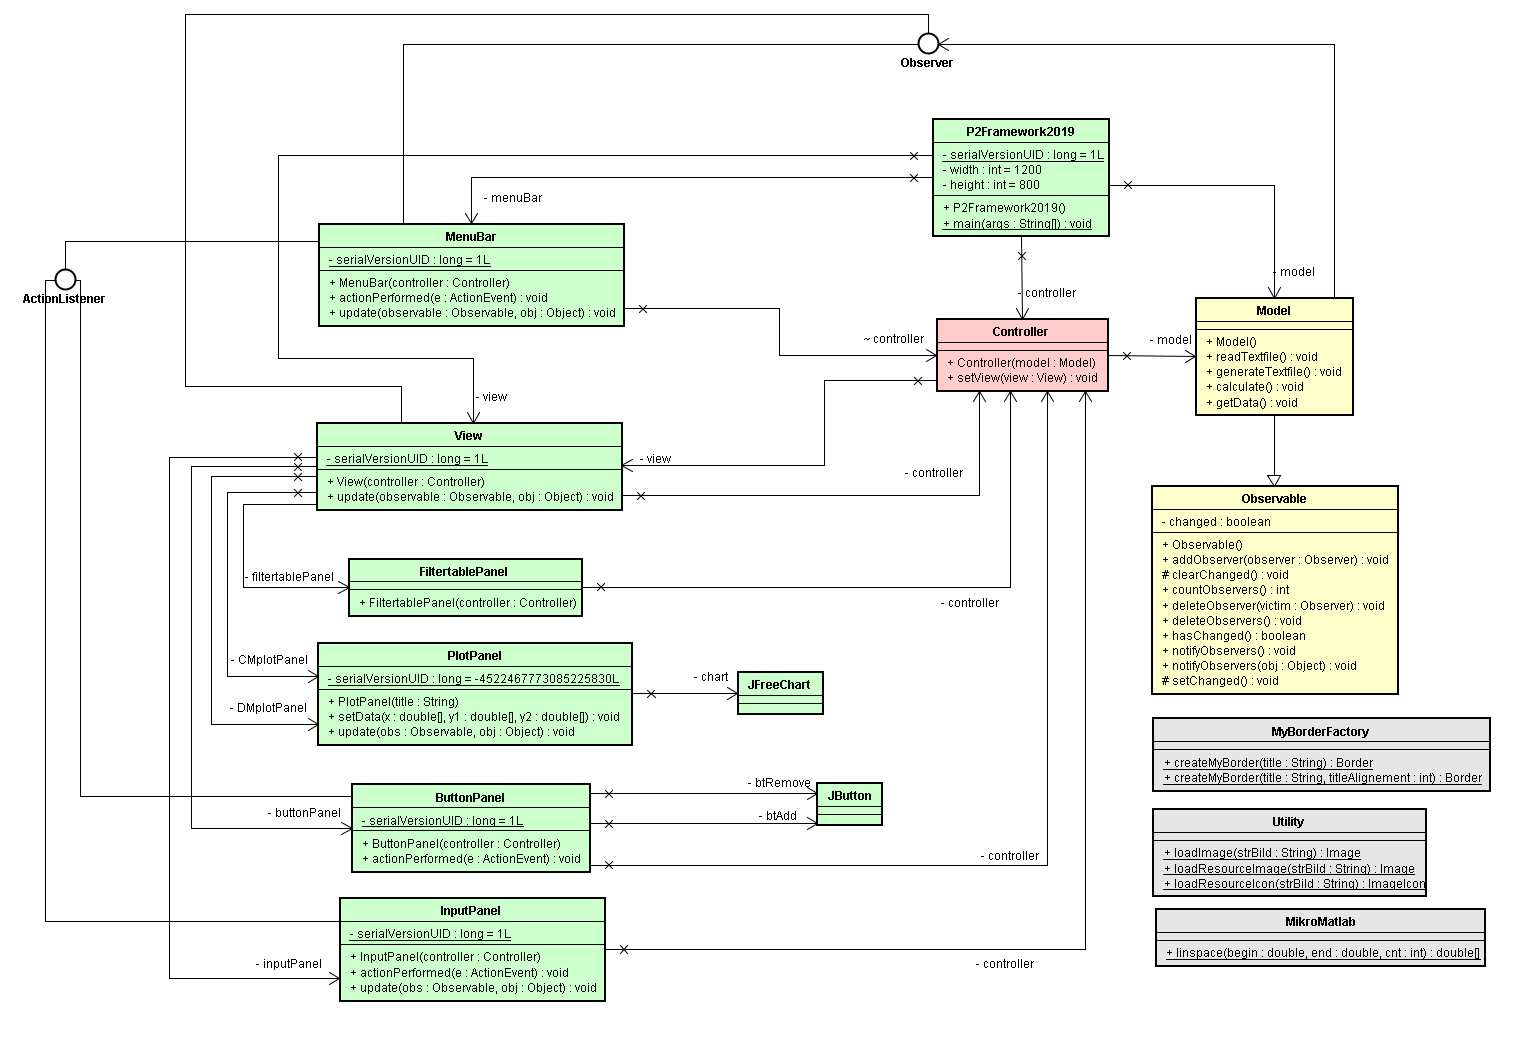
\includegraphics[width=16cm]{Klassendiagramm.png}
	\caption{Klassendiagramm}
	\label{fig:Klassendiagramm}
\end{figure} 

\newpage

\subsection{Fachliche Anforderungen} \label{subsubsec:fachlicheanforderungen}

\bigskip
\shorthandoff{"}
\subsubsection{Softwarestruktur} \label{subsubsec:Softwarestruktur}
Die Software mit Java geschrieben und ist somit Plattformunabhängig. Die Software wird mit dem Model-View-Controller Entwurfsmuster (MVC Design Pattern) \cite{MVCDesignPattern} strukturiert. Durch diese Strukturierung ist es weitgehende möglich die Daten und deren graphische Repräsentation zu trennen. Dies vereinfacht Wartungsarbeiten und die Wiederverwendbarkeit von Programmteile. Die Struktur ist in die drei Teilen Modell(engl. model), Präsentation(engl. view) und Steuerung(engl. controller) unterteilt.

\bigskip
\subsubsection{Mathematische Anforderungen}\label{subsubsec:mathematischeanforderungen}
%TODO Ziel?
Das elektrische Verhalten der CM- und DM-äquivalenten Schaltungen, wird anhand der Streuparameter $S_{21}$ beschrieben. Um den Streuparameter $S_{21}$ zu bestimmen, werden die einzelnen Schaltungsteile in Form von A-Matrixen dargestellt. Diese werden wiederum durch Kaskadieren zu einer A-Matrix der Gesamtschaltungen  zusammengeführt. Der Streuparameter $S_{21}$ wird somit aus der A-Matrix dargestellt. Durch den $S_{21}$ ist durch die Definition die Einfügungsdämfung gegeben. Alle Berechnungen in Java werden zudem in Matlab berechnet, wie auch in der Simulationssoftware MPLAB Mindi simuliert. Dies dient der Verifizierung der Berechnungen in Java.
\bigskip
\subsubsection{Berechnungszeit}\label{subsubsec:berechnungszeit}
Um die erwünschte Berechnungszeit zu erreichen werden die Berechnungen in eigenen Threads ausgeführt. Somit werden "Freezes" im Programm verhindert und mehrere Berechnungen können gleichzeitig ablaufen. 
\bigskip
\subsubsection{Verstellbarkeit der Parameter}\label{subsubsec:verstellbarkeitderparameter}
Eine der Kernfunktionen des Programms besteht darin, dass die Parameter verändert werden können um ihren Einfluss auf die Eingangsdämpfung zu erkennen. Die Parameter sollen um bis +/- 30\% verändert werden können. Da wir hauptsächlich die Auswirkungen graphisch darstellen und analysieren wollen und mit die Veränderungen nicht andauernd eingetippt werden müssen, greifen wir mithilfe eines Schiebereglers darauf zu. 
\bigskip
\subsubsection{Unterscheidung von CM und DM}\label{subsubsec:unterschiedCmDm}
Die zweite Kernfunktion des Programms liegt in der graphischen Anzeige der Berechnungen als Dämpfung in Abhängigkeit der Zeit. Dabei ist die Vorgabe, dass wir einen Plot zum Differential-Mode und einen zum Common-Mode erhalten.
		
\bigskip
\subsubsection{Monte-Carlo Analyse}\label{subsubsec:montecarlo}
Als zusätzliche Simulationsmöglichkeit soll die sog. Monte-Carlo-Analyse implementiert werden. Mit dieser Analyse wird die Auswirkung der Toleranz eines einzelnen Parameters ausgewertet. 
		
		
\subsection{Graphische Anforderungen} \label{subsec:graphischeanforderungen}

\bigskip
\subsubsection{Visualisierung der Schaltungen} \label{subsubsec:visualisierungderschaltungen}
Als generelle Hilfestellung soll das Programm dazu in der Lage sein, das Elektronische Schema der jeweilig Simulierten Schaltung anzuzeigen.
\bigskip
\subsubsection{Eingabemöglichkeiten}\label{subsubsec:eingabemöglichkeiten}
Da wir  die Auswirkungen hauptsächlich graphisch darstellen und analysieren wollen, und damit die Veränderungen nicht andauernd eingetippt werden müssen, greifen wir mithilfe eines Schiebereglers darauf zu.
\bigskip
\subsubsection{Mehrere Plots}\label{subsubsec:mehrereplots}
Das Programm hat seine Vorteile im direkten Vergleich von mehreren Simulationen. So können mehrere Filterprofile gleichzeitig im Plot angezeigt und verglichen werden.
\bigskip
\subsubsection{Frequenbereich}\label{subsubsec:frequenzbereich}
Da das Frequenzspektrum sehr weit ist werden die Plots logarithmisch zur Frequenzachse dargestellt. Sie werden farblich in 3 Bereiche unterteilt.
\bigskip
\subsubsection{Auslagern eines Plots}\label{subsubsec:auslagerneinesplots}
Damit die Bedienung intuitiver gestaltet wird soll es möglich sein die Plot-Fenster aus dem Frame auszulagern um sie beispielsweise zu Vergrössern. 
		

\subsection{Anforderungen an die Bedienung} \label{subsec:bedienungsanforderungen}

\bigskip
\subsubsection{Speicherverwaltung}  \label{subsubsec:speicherverwaltung}
Um einen wirklichen Mehrwert zu schaffen soll die Software die Möglichkeit erhalten, eingestellte Filterprofile abzuspeichern und diese auch nach einem Neustart des Programms wieder zu verwenden. Ebenfalls soll es möglich sein die Plots als Bild, oder PDF-Datei zu exportieren um sie zu verwenden.
\bigskip
\subsubsection{Bedienungshilfen}\label{subsubsec:bedienungshilfen}
Um den User vor Fehleingaben zu schützen verwenden wir die von Herr Gut zur Verfügung gestellten Klassen. diese (TODO:Haben wir überhaupt die Möglichkeit etwas einzugeben?^^)
Sämtliche Funktionen des Programms sind ebenfalls in einem Menu und mithilfe von Shortcuts aufrufbar.

\shorthandon{"}

\subsection{Umsetzung im GUI}\label{subsec:umsetzungimgui}
%TODO Bilder vom Menu noch hier einfügen. die 3 bilder nebeneinandr
In der Abbildung ref{fig:GUI} ist der Aufbau der GUI ersichtlich.

\begin{figure}[H]
	\centering
	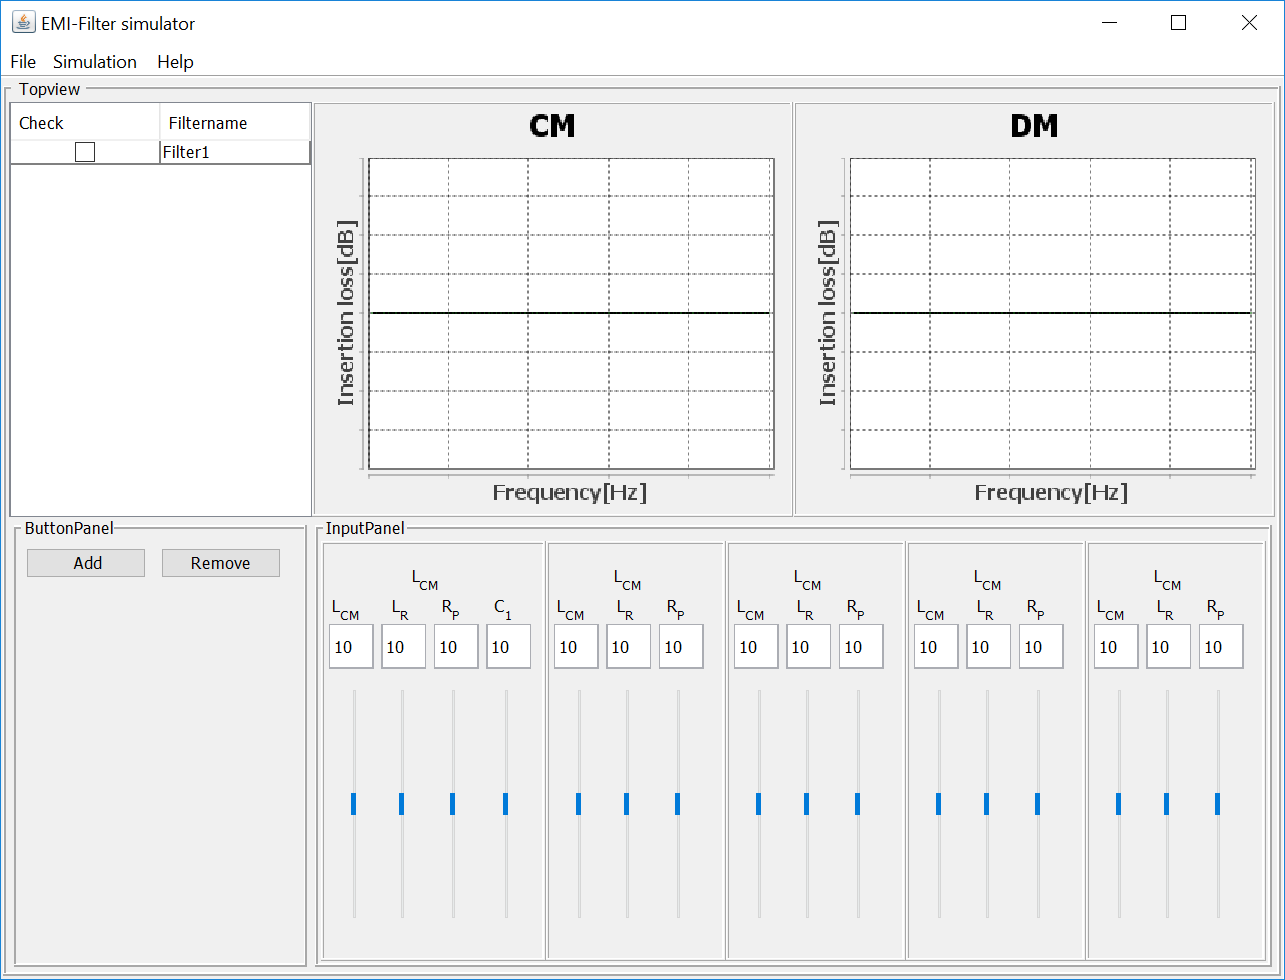
\includegraphics[width=10cm]{GUI.png}
	\caption{GUI}
	\label{fig:GUI}
\end{figure}

\paragraph{Eingabefenster}
Das Eingabefenster stellt die Benutzeroberfläche für die in den Kapitel \ref{subsubsec:auslagerneinesplots} und \ref{subsubsec:eingabemöglichkeiten} beschriebene Anforderungen zur Verfügung.

\paragraph{CM und DM Plot}
Der CM und DM Plot stellt die Benutzeroberfläche für die in den Kapitel \ref{subsubsec:verstellbarkeitderparameter}, \ref{subsubsec:frequenzbereich}, \ref{subsubsec:mehrereplots} und \ref{subsubsec:unterschiedCmDm} beschriebene Anforderungen zur Verfügung.

\paragraph{Filtertabelle}
Die Filtertabelle stellt die Benutzeroberfläche für die in den Kapitel \ref{subsubsec:mehrereplots} und \ref{subsubsec:speicherverwaltung} beschriebene Anforderungen zur Verfügung.

\paragraph{Buttonfenster}
Das Buttonfenster stellt die Benutzeroberfläche für die im Kapitel \ref{subsubsec:mehrereplots} beschriebene Anforderung zur Verfügung.

\paragraph{File}
Der Menupunkt File stellt die Benutzeroberfläche für die im Kapitel \ref{subsubsec:speicherverwaltung} beschriebene Anforderung zur Verfügung.

\paragraph{Simulation}
Der Menupunkt Simulation stellt die Benutzeroberfläche für die im Kapitel \ref{subsubsec:montecarlo} beschriebene Anforderung zur Verfügung.

\paragraph{Help}
Der Menupunkt Help stellt die Benutzeroberfläche für die im Kapitel \ref{subsubsec:bedienungshilfen} beschriebene Anforderung zur Verfügung.


% Auskommentiert. 
\begin{comment}
\subsubsection{Eingabefenster} \label{subsubsec:eingabefenster}

Das Eingabefenster ist dazu da, die einzelnen parasitären Filterparameter einzustellen und die Toleranz von ± 30\% mit einem Schieberegler zu variieren (F6, Tabelle:\ref{tab:ziele}) . Die  Textfelder werden vor Fehleingaben geschützt (B1, Tabelle:\ref{tab:ziele}) und unterstützt spezielle Eingabeformen (z.B 10 milli=10m) (G2, Tabelle:\ref{tab:ziele})

\subsubsection{CM/DM Plot} \label{subsubsec:CM_DMplot}

Um die Berechnungen zu visualisieren werden 2 Plots für CM und DM verwendet(G4, Tabelle:\ref{tab:ziele}) Die Plots sind für die bessere Darstellung in 3 Frequenzbereiche aufgeteilt:0 kHz bis 500 kHz, 500 kHz bis 5 MHz und 5 MHz bis 30 MHz(G3, Tabelle:\ref{tab:ziele}). Mit einem Rechtsklick auf den Plot können verschiedene Optionen ausgewählt werden. So können die Eigenschaften (Farbe, Darstellung, Schrift usw.) und der Zoom individuell eingestellt werden(Fehlt bei Zielen). Der Plot kann auch direkt in eine .png Datei abgespeichert oder gedruckt werden(B2, Tabelle:\ref{tab:ziele}). Diese Optionen sind in der Abbildung \ref{fig:PlotSettings} ersichtlich.

\begin{figure}[H]
	\centering
	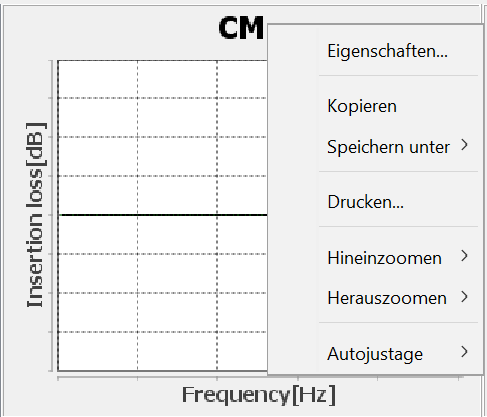
\includegraphics[width=4cm]{PlotSettings.png}
	\caption{Ploteinstellungen}
	\label{fig:PlotSettings}
\end{figure} 


%\subsubsection{Filtertabelle} \label{subsubsec:filtertabelle}
\subsubsection{Speicherverwaltung} \label{subsubsec:speicherverwaltung}

Für das Wunschziel (B3, Tabelle:\ref{tab:ziele}) kann in einer Filtertabelle alle erstellte Filterprofile dargestellt und verwaltet werden.  Mit einer Checkbox können einzelne Profile im Plot aus- bzw. eingeblendet werden. Zudem kann bei jedem Filterprofil einen Namen hinzugefügt werden. Die Werte der parasitären Filterparameter des ausgewählten Filterprofils werden in das Eingabefenster geladen und können dort verändert werden. Mit den Shortcuts Backspace and Delete können ausgewählte Profile gelöscht werden.

\subsubsection{Buttonfenster} \label{subsubsec:buttonfenster}

Im Buttonfenster können Filterprofile in die Filtertabelle geladen oder entfernt werden. (TODO:Zielverweis) Mit dem Button Add werden die eingegebene parasitären Filterparameter in einem neuen Filterprofil gespeichert. Mit dem Button Remove wird das ausgewählte Filterprofil gelöscht. Der Button dient als alternative zu den Shortcuts.


\subsubsection{Menu} \label{subsubsec:menu}

Im Menu können verschiedene Optionen ausgewählt werden. Diese sind ebenfalls alle mit einem Shortcut aufrufbar. (TODO:Zielverweis Ziel Menu)

\bigskip
\shorthandoff{"}
\paragraph{File} \label{para:file}
Im Menupunkt "File" können Filterprofile gespeichert und geladen werden. (B4, Tabelle:\ref{tab:ziele}) Bei beiden Optionen wird der Explorer geöffnet um die .txt Datei im gewählten Verzeichnis abzulegen oder zu holen. In der Option Exit kann das Programm geschlossen werden. Dieser Menupunkt ist in der Abbildung \ref{fig:GUIFile} \nameref{fig:GUIFile} dargestellt.

\begin{figure}[H]
	\centering
	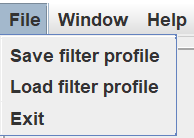
\includegraphics[width=4cm]{GUIFile.png}
	\caption{Menuoption File}
	\label{fig:GUIFile}
\end{figure}

\bigskip

\paragraph{Simulation} \label{para:simulation}
Im Menupunkt "Simulation" kann die Simulationsart Monte Carlo ausgewählt werden(F8, Tabelle:\ref{tab:ziele}). Es öffnet sich ein neues Fenster in dem der Parameter, die Toleranz und die Anzahl Messungen eingestellt werden kann. Dieser Menupunkt ist in der Abbildung \ref{fig:GUISimulation} dargestellt.

\begin{figure}[H]
	\centering
	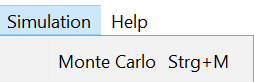
\includegraphics[width=4cm]{GUISimulation.png}
	\caption{Menuoption Simulation}
	\label{fig:GUISimulation}
\end{figure}


\paragraph{Help} \label{para:Help}
Im Menupunkt "Help" können die beiden CM- und DM äquivalenten Schaltungsmodelle, die zur Berechnung verwendet werden, in einem seperaten Fenster dargestellt werden(G5, Tabelle:\ref{tab:ziele}). Dieser Menupunkt ist in der Abbildung \ref{fig:GUIHelp} \nameref{fig:GUIHelp} dargestellt.

\begin{figure}[H]
	\centering
	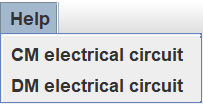
\includegraphics[width=4cm]{GUIHelp.png}
	\caption{Menuoption Help}
	\label{fig:GUIHelp}
\end{figure}
\shorthandon{"}

\end{comment}


\subsection{Libraries} \label{subsec:Libraries}

In der Software werden folgende Libraries verwendet:

\textbf{Swing}: Mit dem vorinstallierten Swing Framework von Java wird die GUI aufgebaut.
\textbf{JFreeChart}: Die Berechnungen werden mit JFreeChart grafisch also Plot dargestellt. \cite{jfreechart}
\textbf{Apache Math Commons} Die Apache Math Commons Library beinhaltet wichtige Mathematikfunktionen, wie rechnen mit Komplexen Zahlen usw. \cite{apache}
\textbf{Engineering Text Fields} Die von Prof. Dr. Richard Gut zur Verfügung gestellte Klasse verhindert Fehleingaben und vereinfacht die Eingabe von Zahlen (nano,piko...)

\newpage